% Options for packages loaded elsewhere
\PassOptionsToPackage{unicode}{hyperref}
\PassOptionsToPackage{hyphens}{url}
\PassOptionsToPackage{dvipsnames,svgnames,x11names}{xcolor}
%
\documentclass[
  ignorenonframetext,
]{beamer}
\usepackage{pgfpages}
\setbeamertemplate{caption}[numbered]
\setbeamertemplate{caption label separator}{: }
\setbeamercolor{caption name}{fg=normal text.fg}
\beamertemplatenavigationsymbolsempty
% Prevent slide breaks in the middle of a paragraph
\widowpenalties 1 10000
\raggedbottom

\usepackage{amsmath,amssymb}
\usepackage{iftex}
\ifPDFTeX
  \usepackage[T1]{fontenc}
  \usepackage[utf8]{inputenc}
  \usepackage{textcomp} % provide euro and other symbols
\else % if luatex or xetex
  \usepackage{unicode-math}
  \defaultfontfeatures{Scale=MatchLowercase}
  \defaultfontfeatures[\rmfamily]{Ligatures=TeX,Scale=1}
\fi
\usepackage{lmodern}
\usetheme[]{AnnArbor}
\usecolortheme{dolphin}
\usefonttheme{structurebold}
\ifPDFTeX\else  
    % xetex/luatex font selection
\fi
% Use upquote if available, for straight quotes in verbatim environments
\IfFileExists{upquote.sty}{\usepackage{upquote}}{}
\IfFileExists{microtype.sty}{% use microtype if available
  \usepackage[]{microtype}
  \UseMicrotypeSet[protrusion]{basicmath} % disable protrusion for tt fonts
}{}
\makeatletter
\@ifundefined{KOMAClassName}{% if non-KOMA class
  \IfFileExists{parskip.sty}{%
    \usepackage{parskip}
  }{% else
    \setlength{\parindent}{0pt}
    \setlength{\parskip}{6pt plus 2pt minus 1pt}}
}{% if KOMA class
  \KOMAoptions{parskip=half}}
\makeatother
\usepackage{xcolor}
\newif\ifbibliography
\setlength{\emergencystretch}{3em} % prevent overfull lines
\setcounter{secnumdepth}{-\maxdimen} % remove section numbering


\providecommand{\tightlist}{%
  \setlength{\itemsep}{0pt}\setlength{\parskip}{0pt}}\usepackage{longtable,booktabs,array}
\usepackage{calc} % for calculating minipage widths
\usepackage{caption}
% Make caption package work with longtable
\makeatletter
\def\fnum@table{\tablename~\thetable}
\makeatother
\usepackage{graphicx}
\makeatletter
\def\maxwidth{\ifdim\Gin@nat@width>\linewidth\linewidth\else\Gin@nat@width\fi}
\def\maxheight{\ifdim\Gin@nat@height>\textheight\textheight\else\Gin@nat@height\fi}
\makeatother
% Scale images if necessary, so that they will not overflow the page
% margins by default, and it is still possible to overwrite the defaults
% using explicit options in \includegraphics[width, height, ...]{}
\setkeys{Gin}{width=\maxwidth,height=\maxheight,keepaspectratio}
% Set default figure placement to htbp
\makeatletter
\def\fps@figure{htbp}
\makeatother
% definitions for citeproc citations
\NewDocumentCommand\citeproctext{}{}
\NewDocumentCommand\citeproc{mm}{%
  \begingroup\def\citeproctext{#2}\cite{#1}\endgroup}
\makeatletter
 % allow citations to break across lines
 \let\@cite@ofmt\@firstofone
 % avoid brackets around text for \cite:
 \def\@biblabel#1{}
 \def\@cite#1#2{{#1\if@tempswa , #2\fi}}
\makeatother
\newlength{\cslhangindent}
\setlength{\cslhangindent}{1.5em}
\newlength{\csllabelwidth}
\setlength{\csllabelwidth}{3em}
\newenvironment{CSLReferences}[2] % #1 hanging-indent, #2 entry-spacing
 {\begin{list}{}{%
  \setlength{\itemindent}{0pt}
  \setlength{\leftmargin}{0pt}
  \setlength{\parsep}{0pt}
  % turn on hanging indent if param 1 is 1
  \ifodd #1
   \setlength{\leftmargin}{\cslhangindent}
   \setlength{\itemindent}{-1\cslhangindent}
  \fi
  % set entry spacing
  \setlength{\itemsep}{#2\baselineskip}}}
 {\end{list}}
\usepackage{calc}
\newcommand{\CSLBlock}[1]{\hfill\break\parbox[t]{\linewidth}{\strut\ignorespaces#1\strut}}
\newcommand{\CSLLeftMargin}[1]{\parbox[t]{\csllabelwidth}{\strut#1\strut}}
\newcommand{\CSLRightInline}[1]{\parbox[t]{\linewidth - \csllabelwidth}{\strut#1\strut}}
\newcommand{\CSLIndent}[1]{\hspace{\cslhangindent}#1}

\usepackage{booktabs}
\usepackage{longtable}
\usepackage{array}
\usepackage{multirow}
\usepackage{wrapfig}
\usepackage{float}
\usepackage{colortbl}
\usepackage{pdflscape}
\usepackage{tabu}
\usepackage{threeparttable}
\usepackage{threeparttablex}
\usepackage[normalem]{ulem}
\usepackage{makecell}
\usepackage{xcolor}

% logo
\titlegraphic{
\includegraphics[width=4cm]{000_logos/logo-blue-vertical}}
\logo{\ifnum\thepage>1
\includegraphics[width=0.5cm]{000_logos/logo-blue-vertical}\fi}

% UMNG: Manual de image institucional

% Colors

% Umng
\definecolor{yellow}{HTML}{fdc600}
\definecolor{red}{HTML}{ee2a24}

% Estudios a Distancia
\definecolor{blue1}{HTML}{12245b}
\definecolor{blue2}{HTML}{767ca6}
\definecolor{blue3}{HTML}{cad2ec}

% Modify items
\setbeamercolor{palette primary}{bg=blue3}
\setbeamercolor{palette tertiary}{bg=blue1}
\setbeamercolor{frametitle}{bg=yellow}

% Hyperlinks
\hypersetup{
  linkcolor=red,
  citecolor=red
}

\makeatletter
\@ifpackageloaded{caption}{}{\usepackage{caption}}
\AtBeginDocument{%
\ifdefined\contentsname
  \renewcommand*\contentsname{Table of contents}
\else
  \newcommand\contentsname{Table of contents}
\fi
\ifdefined\listfigurename
  \renewcommand*\listfigurename{List of Figures}
\else
  \newcommand\listfigurename{List of Figures}
\fi
\ifdefined\listtablename
  \renewcommand*\listtablename{List of Tables}
\else
  \newcommand\listtablename{List of Tables}
\fi
\ifdefined\figurename
  \renewcommand*\figurename{Figure}
\else
  \newcommand\figurename{Figure}
\fi
\ifdefined\tablename
  \renewcommand*\tablename{Table}
\else
  \newcommand\tablename{Table}
\fi
}
\@ifpackageloaded{float}{}{\usepackage{float}}
\floatstyle{ruled}
\@ifundefined{c@chapter}{\newfloat{codelisting}{h}{lop}}{\newfloat{codelisting}{h}{lop}[chapter]}
\floatname{codelisting}{Listing}
\newcommand*\listoflistings{\listof{codelisting}{List of Listings}}
\makeatother
\makeatletter
\makeatother
\makeatletter
\@ifpackageloaded{caption}{}{\usepackage{caption}}
\@ifpackageloaded{subcaption}{}{\usepackage{subcaption}}
\makeatother

\ifLuaTeX
\usepackage[bidi=basic]{babel}
\else
\usepackage[bidi=default]{babel}
\fi
\babelprovide[main,import]{english}
% get rid of language-specific shorthands (see #6817):
\let\LanguageShortHands\languageshorthands
\def\languageshorthands#1{}
\ifLuaTeX
  \usepackage{selnolig}  % disable illegal ligatures
\fi
\usepackage{bookmark}

\IfFileExists{xurl.sty}{\usepackage{xurl}}{} % add URL line breaks if available
\urlstyle{same} % disable monospaced font for URLs
\hypersetup{
  pdftitle={Production and Income II},
  pdfauthor={Luis Francisco Gómez López},
  pdflang={en},
  colorlinks=true,
  linkcolor={Maroon},
  filecolor={Maroon},
  citecolor={Blue},
  urlcolor={Blue},
  pdfcreator={LaTeX via pandoc}}


\title{Production and Income II}
\author{Luis Francisco Gómez López}
\date{2024-07-13}
\institute{FAEDIS}

\begin{document}
\frame{\titlepage}

\renewcommand*\contentsname{Table of contents}
\begin{frame}[allowframebreaks]
  \frametitle{Table of contents}
  \tableofcontents[hideallsubsections]
\end{frame}

\section{Please Read Me}\label{please-read-me}

\begin{frame}{}
\phantomsection\label{section}
\begin{itemize}
\item
  Check the message \textbf{Welcome greeting} published in the News
  Bulletin Board.
\item
  Dear student please edit your profile uploading a photo where your
  face is clearly visible.
\item
  The purpose of the virtual meetings is to answer questions and not to
  make a summary of the study material.
\item
  This presentation is based on
  (\citeproc{ref-cardenas_introduccion_2020}{Cardenas 2020, chap. 2})
\end{itemize}
\end{frame}

\section{Purpose}\label{purpose}

\begin{frame}{}
\phantomsection\label{section-1}
Understand how production is measured using the concept of Gross
Domestic Product (GDP)
\end{frame}

\section{Inflation adjustments in
GPD}\label{inflation-adjustments-in-gpd}

\begin{frame}{}
\phantomsection\label{section-2}
\begin{itemize}
\item
  Initially the Gross Domestic Product is expressed in current Local
  Currency Units (LCU) which is the sum of monetary values
\item
  A particular monetary value is the product of a quantity and a unit
  price
\item
  A change in the level of Gross Domestic Product, measure in current
  LCU, is a combination of changes in quantities and prices

  \begin{itemize}
  \item
    Inflation adjustments, applied to GDP, \textbf{try} to eliminate the
    changes of prices
  \item
    There are 2 approaches to make inflation adjustments
    (\citeproc{ref-abs_demystifying_2003}{ABS 2003}):

    \begin{itemize}
    \tightlist
    \item
      \textbf{Constant price estimates}
    \item
      \textbf{Chain volume measures}
    \end{itemize}
  \end{itemize}
\end{itemize}
\end{frame}

\begin{frame}{}
\phantomsection\label{section-3}
\begin{itemize}
\item
  \textbf{Chain volume measures} is the alternative used by the
  Departamento Administrativo Nacional de Estadística (DANE) to make
  inflation adjustments

  \begin{itemize}
  \item
    A gentle introduction to this approach is explained in
    (\citeproc{ref-abs_demystifying_2003}{ABS 2003})
  \item
    The monetary values adjusted using \textbf{chain volume measures}
    are not additive. This means that the sum of the components of an
    aggregate is not necessarily equal to the aggregate

    \begin{itemize}
    \tightlist
    \item
      In addition to the values adjusted using \textbf{chain volume
      measures}, DANE reports a value known as statistical discrepancy
      because of non additivity
    \end{itemize}
  \end{itemize}
\end{itemize}
\end{frame}

\begin{frame}{}
\phantomsection\label{section-4}
\begin{table}

\caption{\label{tbl-expenditure-approach-chain-volume}Expenditure/Final
demand approach using chain volume measures and expressed in thousands
of millions (Colombia)}

\centering{

\centering\begingroup\fontsize{7}{9}\selectfont

\begin{threeparttable}
\begin{tabular}{lrrr}
\toprule
\textbf{Concepto} & \textbf{2015} & \textbf{2022\textsuperscript{a}} & \textbf{2023\textsuperscript{b}}\\
\midrule
\cellcolor[HTML]{18BC9C}{Gasto de consumo final individual de los hogares y las ISFLH\textsuperscript{c}} & \cellcolor[HTML]{18BC9C}{551013} & \cellcolor[HTML]{18BC9C}{740299} & \cellcolor[HTML]{18BC9C}{746541}\\
\hspace{1em}Gasto de consumo final individual de los hogares & 547843 & 736931 & NA\\
\hspace{1em}Gasto de consumo final de las ISFLH\textsuperscript{c} & 3170 & 3404 & NA\\
\cellcolor[HTML]{18BC9C}{Gasto de consumo final del gobierno general} & \cellcolor[HTML]{18BC9C}{119188} & \cellcolor[HTML]{18BC9C}{156237} & \cellcolor[HTML]{18BC9C}{158758}\\
\cellcolor[HTML]{18BC9C}{Formación bruta de capital} & \cellcolor[HTML]{18BC9C}{191305} & \cellcolor[HTML]{18BC9C}{198273} & \cellcolor[HTML]{18BC9C}{147015}\\
\addlinespace
\cellcolor[HTML]{18BC9C}{Exportaciones} & \cellcolor[HTML]{18BC9C}{125936} & \cellcolor[HTML]{18BC9C}{133496} & \cellcolor[HTML]{18BC9C}{138021}\\
\cellcolor[HTML]{FF7F00}{Importaciones} & \cellcolor[HTML]{FF7F00}{182750} & \cellcolor[HTML]{FF7F00}{253174} & \cellcolor[HTML]{FF7F00}{215163}\\
\cellcolor[HTML]{e31a1c}{Producto interno bruto} & \cellcolor[HTML]{e31a1c}{804692} & \cellcolor[HTML]{e31a1c}{972298} & \cellcolor[HTML]{e31a1c}{978233}\\
\cellcolor[HTML]{CAB2D6}{Discrepancia estadística} & \cellcolor[HTML]{CAB2D6}{0} & \cellcolor[HTML]{CAB2D6}{-3207} & \cellcolor[HTML]{CAB2D6}{2786}\\
\bottomrule
\end{tabular}
\begin{tablenotes}
\item Source: DANE - Cuentas Nacionales Anuales - Producto Interno Bruto (PIB) - Series encadenadas de volumen con año de referencia 2015
\item Last update: 2024-06-28
\item[a] Provisional data
\item[b] Preliminary data
\item[c] Instituciones sin fines de lucro que sirven a los hogares
\end{tablenotes}
\end{threeparttable}
\endgroup{}

}

\end{table}%
\end{frame}

\begin{frame}{}
\phantomsection\label{section-5}
\begin{table}

\caption{\label{tbl-expenditure-approach-current-prices}Expenditure/Final
demand approach using current prices and expressed in thousands of
millions (Colombia)}

\centering{

\centering\begingroup\fontsize{7}{9}\selectfont

\begin{threeparttable}
\begin{tabular}{lrrr}
\toprule
\textbf{Concepto} & \textbf{2015} & \textbf{2022\textsuperscript{a}} & \textbf{2023\textsuperscript{b}}\\
\midrule
\cellcolor[HTML]{18BC9C}{Gasto de consumo final individual de los hogares y las ISFLSH\textsuperscript{c}} & \cellcolor[HTML]{18BC9C}{551013} & \cellcolor[HTML]{18BC9C}{1085690} & \cellcolor[HTML]{18BC9C}{1202350}\\
\hspace{1em}Gasto de consumo final individual de los hogares & 547843 & 1080441 & 1196277\\
\hspace{1em}Gasto de consumo final de las ISFLH\textsuperscript{c} & 3170 & 5249 & 6073\\
\cellcolor[HTML]{18BC9C}{Gasto de consumo final del gobierno general} & \cellcolor[HTML]{18BC9C}{119188} & \cellcolor[HTML]{18BC9C}{205744} & \cellcolor[HTML]{18BC9C}{231997}\\
\cellcolor[HTML]{18BC9C}{Formación bruta de capital} & \cellcolor[HTML]{18BC9C}{191305} & \cellcolor[HTML]{18BC9C}{290196} & \cellcolor[HTML]{18BC9C}{213891}\\
\addlinespace
\cellcolor[HTML]{18BC9C}{Exportaciones} & \cellcolor[HTML]{18BC9C}{125936} & \cellcolor[HTML]{18BC9C}{297374} & \cellcolor[HTML]{18BC9C}{280484}\\
\cellcolor[HTML]{FF7F00}{Importaciones} & \cellcolor[HTML]{FF7F00}{182750} & \cellcolor[HTML]{FF7F00}{409213} & \cellcolor[HTML]{FF7F00}{356264}\\
\cellcolor[HTML]{e31a1c}{Producto interno bruto} & \cellcolor[HTML]{e31a1c}{804692} & \cellcolor[HTML]{e31a1c}{1469791} & \cellcolor[HTML]{e31a1c}{1572458}\\
\bottomrule
\end{tabular}
\begin{tablenotes}
\item Source: DANE - Cuentas Nacionales Anuales - Producto Interno Bruto (PIB) - Precios corrientes
\item Last update: 2024-06-28
\item[a] Provisional data
\item[b] Preliminary data
\item[c] Instituciones sin fines de lucro que sirven a los hogares
\end{tablenotes}
\end{threeparttable}
\endgroup{}

}

\end{table}%
\end{frame}

\section{Economics sectors and GDP}\label{economics-sectors-and-gdp}

\begin{frame}{}
\phantomsection\label{section-6}
\begin{table}

\caption{\label{tbl-isic-col-1}ISIC adapted for Colombia
(\citeproc{ref-dane_clasificacion_2022}{DANE 2022, 134--677})}

\centering{

\centering\begingroup\fontsize{9}{11}\selectfont

\begin{tabular}{>{\raggedright\arraybackslash}p{0.3in}>{\raggedright\arraybackslash}p{0.3in}>{\raggedright\arraybackslash}p{3.4in}}
\toprule
\textbf{Section} & \textbf{Division} & \textbf{Description}\\
\midrule
\cellcolor{gray!10}{A} & \cellcolor{gray!10}{01-03} & \cellcolor{gray!10}{Agricultura, ganadería, caza, silvicultura y pesca}\\
B & 05-09 & Explotación de minas y canteras\\
\cellcolor{gray!10}{C} & \cellcolor{gray!10}{10-33} & \cellcolor{gray!10}{Industrias manufactureras}\\
D & 35 & Suministro de electricidad, gas, vapor, y aire acondicionado\\
E & 36-39 & Distribución de agua; evacuación y tratamiento de aguas residuales, gestión de desechos y
\cellcolor{gray!10}{actividades de saneamiento ambiental}\\
\addlinespace
F & 41-43 & Construcción\\
\cellcolor{gray!10}{G} & \cellcolor{gray!10}{45-47} & \cellcolor{gray!10}{Comercio al por mayor y al por menor; reparación de vehículos automotores y motocicletas}\\
H & 49-53 & Transporte y almacenamiento\\
\cellcolor{gray!10}{I} & \cellcolor{gray!10}{55-56} & \cellcolor{gray!10}{Alojamiento y servicios de comida}\\
J & 58-63 & Información y comunicaciones\\
\addlinespace
\cellcolor{gray!10}{K} & \cellcolor{gray!10}{64-66} & \cellcolor{gray!10}{Actividades financieras y de seguros}\\
\bottomrule
\end{tabular}
\endgroup{}

}

\end{table}%
\end{frame}

\begin{frame}{}
\phantomsection\label{section-7}
\begin{table}

\caption{\label{tbl-isic-col-2}ISIC adapted for Colombia
(\citeproc{ref-dane_clasificacion_2022}{DANE 2022, 134--677})}

\centering{

\centering\begingroup\fontsize{9}{11}\selectfont

\begin{threeparttable}
\begin{tabular}{>{\raggedright\arraybackslash}p{0.3in}>{\raggedright\arraybackslash}p{0.3in}>{\raggedright\arraybackslash}p{3.4in}}
\toprule
\textbf{Section} & \textbf{Division} & \textbf{Description}\\
\midrule
\cellcolor{gray!10}{L} & \cellcolor{gray!10}{68} & \cellcolor{gray!10}{Actividades inmobiliarias}\\
M & 69-75 & Actividades profesionales, científicas y técnicas\\
\cellcolor{gray!10}{N} & \cellcolor{gray!10}{77-82} & \cellcolor{gray!10}{Actividades de servicios administrativos y de poyo}\\
O & 84 & Administración pública y defensa; planes de seguridad social de afiliación obligatoria\\
\cellcolor{gray!10}{P} & \cellcolor{gray!10}{85} & \cellcolor{gray!10}{Educación}\\
\addlinespace
Q & 86-88 & Actividades de atención de la salud humana y de asistencia social\\
\cellcolor{gray!10}{R} & \cellcolor{gray!10}{90-93} & \cellcolor{gray!10}{Actividades artísticas, de entretenimiento y recreación}\\
S & 94-96 & Otras actividades de servicios\\
T & 97-98 & Actividades de los hogares en calidad de empleadores; actividades no diferenciadas de los
\cellcolor{gray!10}{hogares individuales como productores de bienes y servicios para uso propio}\\
\cellcolor[HTML]{e31a1c}{U} & \cellcolor[HTML]{e31a1c}{99} & \cellcolor[HTML]{e31a1c}{Actividades de organizaciones y entidades extraterritoriales\textsuperscript{a}}\\
\bottomrule
\end{tabular}
\begin{tablenotes}
\item[a] Because of extraterritoriality, in the context of international law, the production units that belong to this category are not part of the domestic territory
\end{tablenotes}
\end{threeparttable}
\endgroup{}

}

\end{table}%
\end{frame}

\begin{frame}{}
\phantomsection\label{section-8}
\begin{figure}

\centering{

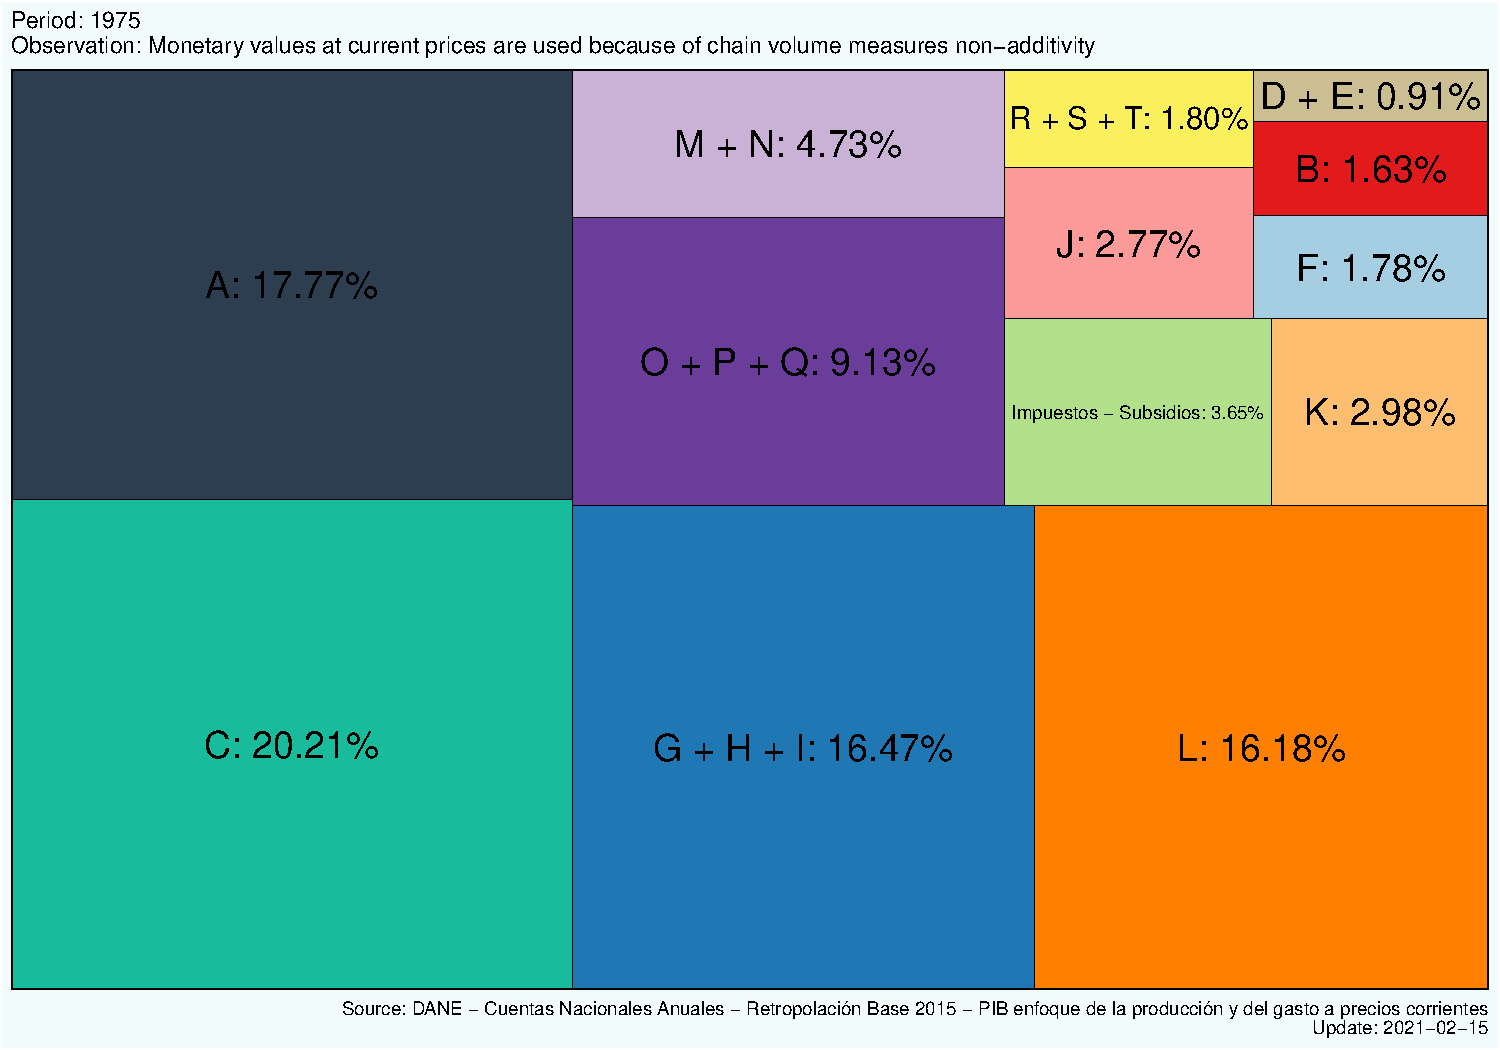
\includegraphics[width=0.85\textwidth,height=\textheight]{002_production_income_II_files/figure-beamer/fig-sectors-share-gdp-col-1975-1.pdf}

}

\caption{\label{fig-sectors-share-gdp-col-1975}Sectors and share in GDP
for Colombia}

\end{figure}%
\end{frame}

\begin{frame}{}
\phantomsection\label{section-9}
\begin{figure}

\centering{

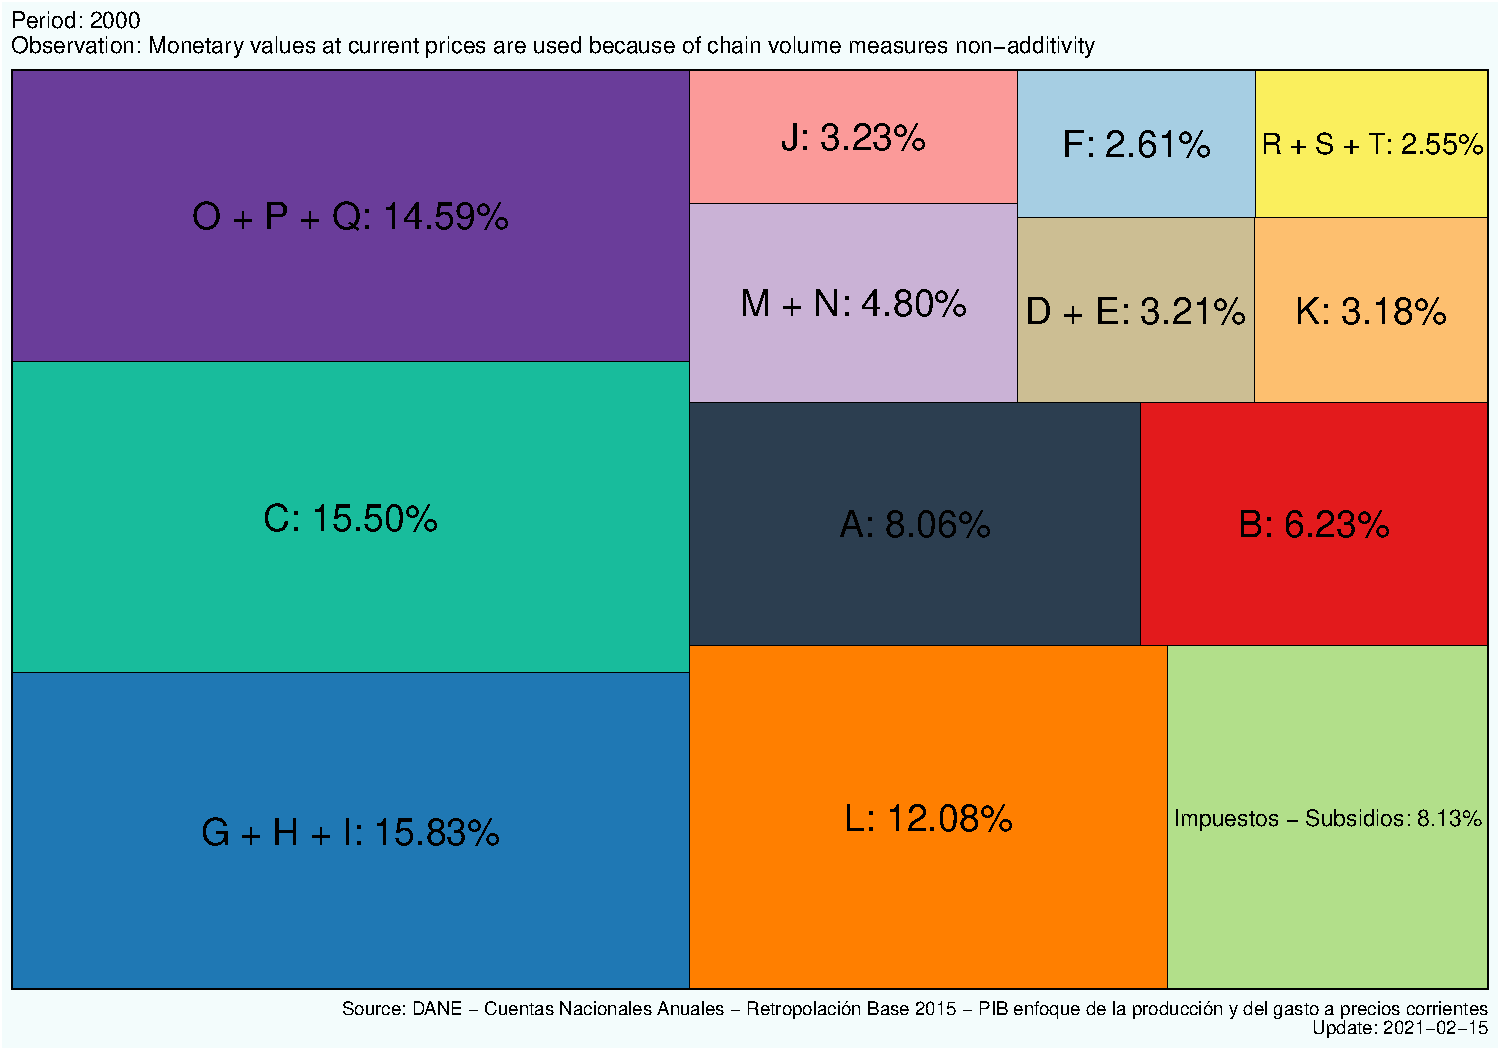
\includegraphics[width=0.85\textwidth,height=\textheight]{002_production_income_II_files/figure-beamer/fig-sectors-share-gdp-col-2000-1.pdf}

}

\caption{\label{fig-sectors-share-gdp-col-2000}Sectors and share in GDP
for Colombia}

\end{figure}%
\end{frame}

\begin{frame}{}
\phantomsection\label{section-10}
\begin{figure}

\centering{

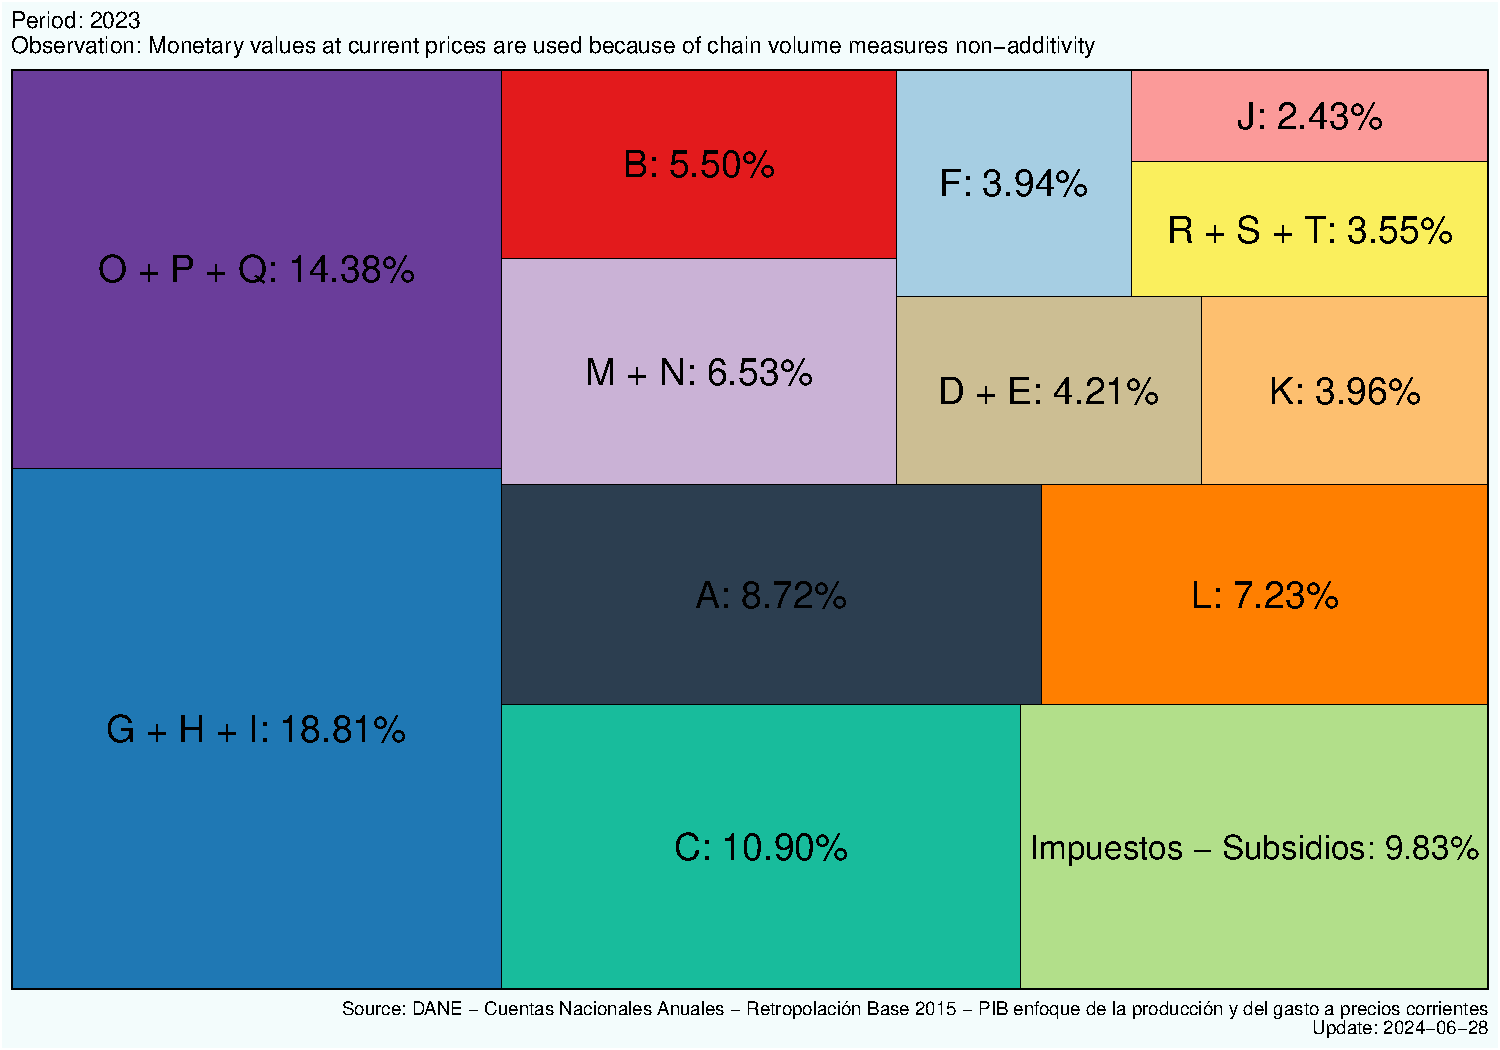
\includegraphics[width=0.85\textwidth,height=\textheight]{002_production_income_II_files/figure-beamer/fig-sectors-share-gdp-col-2021-1.pdf}

}

\caption{\label{fig-sectors-share-gdp-col-2021}Sectors and share in GDP
for Colombia}

\end{figure}%
\end{frame}

\section{Macroeconomic identity}\label{macroeconomic-identity}

\begin{frame}{}
\phantomsection\label{section-11}
\begin{itemize}
\tightlist
\item
  Uses that firms, non-profit institutions, government bodies,
  households and the external sector give to production
\end{itemize}

\small

\[\begin{split}
  \mathbf{Demand}_t  = & \text{Gasto de consumo final individual de los hogares y las ISFLH}_t + \\
  & \text{Gasto de consumo final del gobierno general}_t + \\
  & \text{Formación bruta de capital}_t + \\
  & \text{Exportaciones}_t \\
  = & C_t + G_t + I_t + X_t
  \end{split}\]
\end{frame}

\begin{frame}{}
\phantomsection\label{section-12}
\begin{itemize}
\tightlist
\item
  Aggregate value generated by the production units in a territory, plus
  taxes minus subsidies on products, plus products produced outside the
  territory offered to the territory
\end{itemize}

\[\begin{split}
  \mathbf{Supply}_t  = & \text{Valor agregado bruto}_t + \\
  & \text{Impuestos menos subvenciones sobre los productos}_t + \\
  & \text{Importaciones}_t \\
  = & \text{Producto interno bruto}_t + \\
  & \text{Importaciones}_t \\
  = & GDP_t + M_t
  \end{split}\]
\end{frame}

\begin{frame}{}
\phantomsection\label{section-13}
\[\begin{split}
  \mathbf{Supply}_t & = \mathbf{Demand}_t \\
  GDP_t + M_t & = C_t + G_t + I_t + X_t \\
  GDP_t & = (C_t + G_t + I_t) + (X_t - M_t)
  \end{split}\]
\end{frame}

\begin{frame}{}
\phantomsection\label{section-14}
\begin{figure}

\centering{

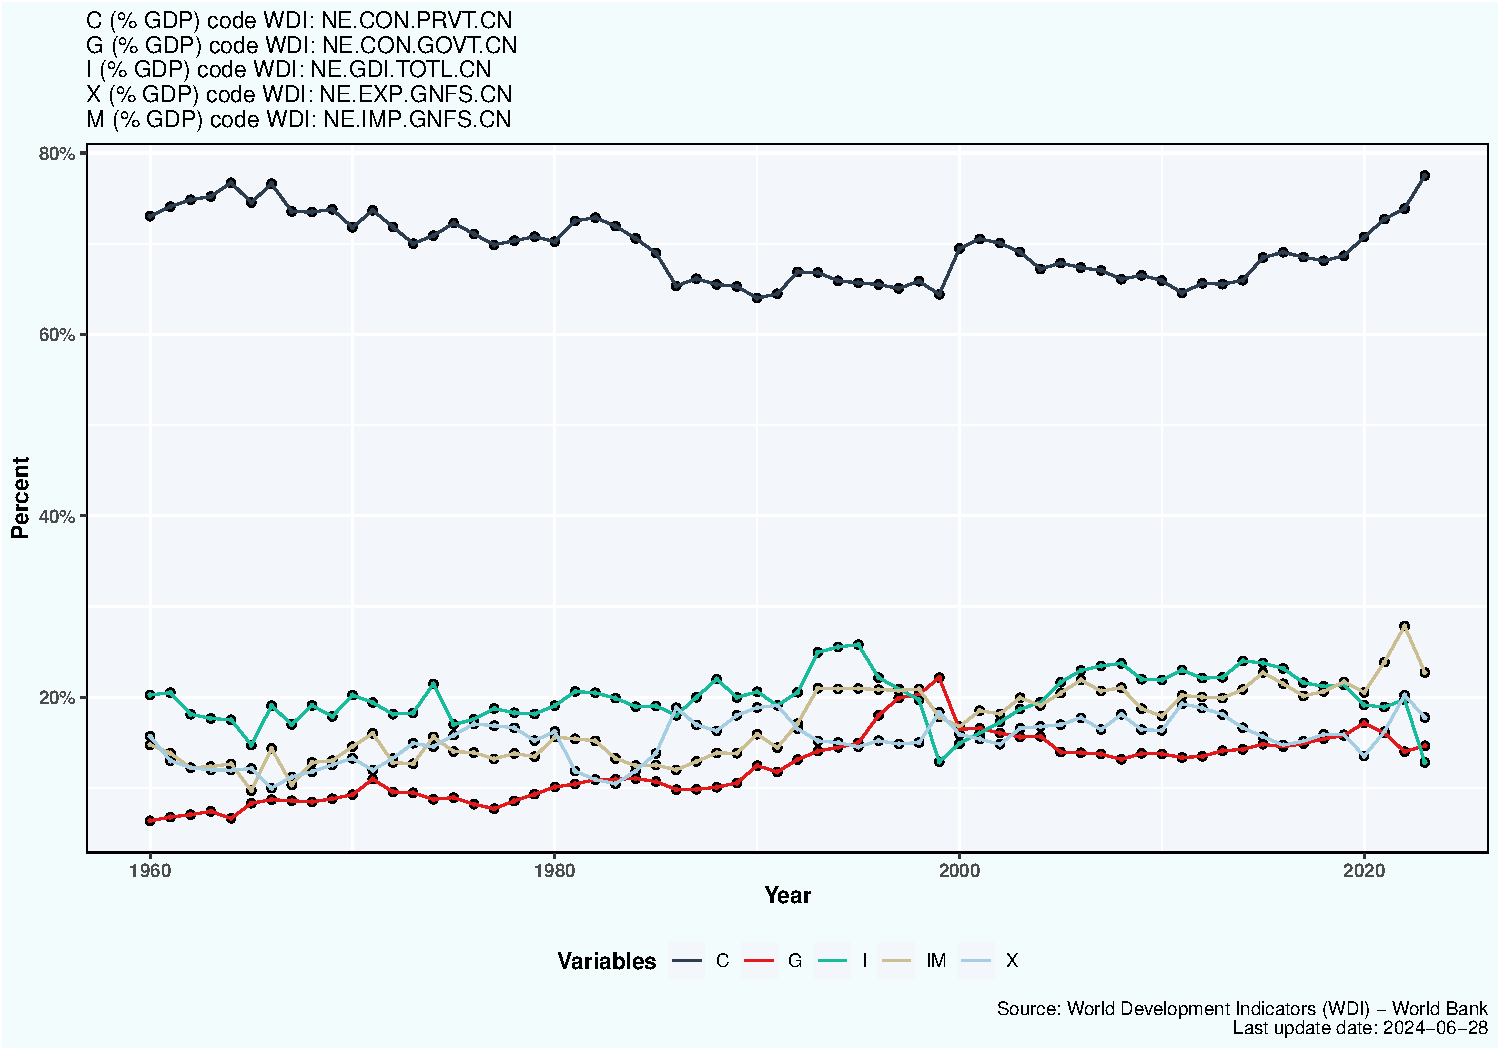
\includegraphics[width=0.85\textwidth,height=\textheight]{002_production_income_II_files/figure-beamer/fig-share-gdp-components-col-1.pdf}

}

\caption{\label{fig-share-gdp-components-col}Share of GDP components in
Colombia}

\end{figure}%
\end{frame}

\section{Resource of interest}\label{resource-of-interest}

\begin{frame}{}
\phantomsection\label{section-15}
If you want a summary about the topic of Gross Domestic Product check
out\footnote<.->{Banco de la República de Colombia - Cátedras de
  Macroeconomía y Banca Central}:

\begin{itemize}
\tightlist
\item
  \url{https://youtu.be/YXTjJSGWnsE}
\end{itemize}
\end{frame}

\section{Acknowledgments}\label{acknowledgments}

\begin{frame}{}
\phantomsection\label{section-16}
\begin{itemize}
\item
  To my family that supports me
\item
  To the taxpayers of Colombia and the
  \href{https://www.umng.edu.co/estudiante}{\textbf{UMNG students}} who
  pay my salary
\item
  To the \href{https://www.business-science.io/}{\textbf{Business
  Science}} and \href{https://www.rfordatasci.com/}{\textbf{R4DS Online
  Learning}} communities where I learn
  \href{https://www.r-project.org/about.html}{\textbf{R}} and
  \href{https://www.python.org/about/}{\textbf{\(\pi\)-thon}}
\item
  To the \href{https://www.r-project.org/contributors.html}{\textbf{R
  Core Team}}, the creators of
  \href{https://rstudio.com/products/rstudio/}{\textbf{RStudio IDE}},
  \href{https://quarto.org/}{\textbf{Quarto}} and the authors and
  maintainers of the packages
  \href{https://CRAN.R-project.org/package=tidyverse}{\textbf{tidyverse}},
  \href{https://CRAN.R-project.org/package=readxl}{\textbf{readxl}},
  \href{https://CRAN.R-project.org/package=knitr}{\textbf{knitr}},
  \href{https://CRAN.R-project.org/package=kableExtra}{\textbf{kableExtra}},
  \href{https://CRAN.R-project.org/package=janitor}{\textbf{janitor}},
  \href{https://CRAN.R-project.org/package=treemapify}{\textbf{treemapify}},
  \href{https://CRAN.R-project.org/package=tidyquant}{\textbf{tidyquant}},
  \href{https://CRAN.R-project.org/package=wbstats}{\textbf{wbstats}}
  and
  \href{https://CRAN.R-project.org/package=tinytex}{\textbf{tinytex}}
  for allowing me to access these tools without paying for a license
\item
  To the \href{https://www.kernel.org/category/about.html}{\textbf{Linux
  kernel community}} for allowing me the possibility to use some
  \href{https://static.lwn.net/Distributions/}{\textbf{Linux
  distributions}} as my main
  \href{https://en.wikipedia.org/wiki/Operating_system}{\textbf{OS}}
  without paying for a license
\end{itemize}
\end{frame}

\section*{References}\label{references}
\addcontentsline{toc}{section}{References}

\begin{frame}[allowframebreaks]{References}
\phantomsection\label{refs}
\begin{CSLReferences}{1}{0}
\bibitem[\citeproctext]{ref-abs_demystifying_2003}
ABS. 2003. {``Demystifying {Chain} {Volume} {Measures}.''} \emph{Western
Australian Statistical Indicators}, March, 16--25.
\url{https://www.ausstats.abs.gov.au/ausstats/subscriber.nsf/0/08CFB1A8C9431C57CA256D030004EE42/$File/13675_mar\%202003.pdf}.

\bibitem[\citeproctext]{ref-cardenas_introduccion_2020}
Cardenas, Mauricio. 2020. \emph{Introducción a La {Economía}
{Colombiana}}. 4th ed. Alfaomega.

\bibitem[\citeproctext]{ref-dane_clasificacion_2022}
DANE. 2022. {``Clasificación {Industrial} {Internacional} {Uniforme} de
Todas Las Actividades Económicas {Revisión} 4 {Adaptada} Para {Colombia}
(2022).''}
\url{https://www.dane.gov.co/files/sen/nomenclatura/ciiu/CIIU_Rev_4_AC2022.pdf}.

\end{CSLReferences}
\end{frame}




\end{document}
